\documentclass[conference]{IEEEtran}
\IEEEoverridecommandlockouts
\usepackage{cite}
\usepackage{amsmath,amssymb,amsfonts}
\usepackage{algorithmic}
\usepackage{graphicx}
\usepackage{textcomp}
\usepackage{xcolor}
\usepackage{booktabs}
\usepackage{multirow}
\usepackage{url}
\def\BibTeX{{\rm B\kern-.05em{\sc i\kern-.025em b}\kern-.08em
    T\kern-.1667em\lower.7ex\hbox{E}\kern-.125emX}}
\begin{document}

\title{An AI-Driven Personalized Sinhala Teaching Assistant for Secondary Education Using Curriculum Aligned Large Language Models}

\author{
\IEEEauthorblockN{Gunasekara K.K.S.\textsuperscript{*}}
\IEEEauthorblockA{\textit{Department of Electrical and} \\
\textit{Information Engineering} \\
\textit{University of Ruhuna}\\
Galle, Sri Lanka \\
gunasekara\_kks\_e23@engug.ruh.ac.lk}
\and
\IEEEauthorblockN{Wijesinghe D.M.A.B.}
\IEEEauthorblockA{\textit{Department of Electrical and} \\
\textit{Information Engineering} \\
\textit{University of Ruhuna}\\
Galle, Sri Lanka \\
wijesinghe\_dma\_e23@engug.ruh.ac.lk}
\and
\IEEEauthorblockN{Akarshana A.N.\textsuperscript{*}}
\IEEEauthorblockA{\textit{Department of Electrical and} \\
\textit{Information Engineering} \\
\textit{University of Ruhuna}\\
Galle, Sri Lanka \\
akarshana\_an\_e23@engug.ruh.ac.lk}
\and
\IEEEauthorblockN{\phantom{Gunasekara K.K.S.\textsuperscript{*}}}
\IEEEauthorblockA{\textit{\phantom{Department of Electrical and}} \\
\textit{\phantom{Information Engineering}} \\
\textit{\phantom{University of Ruhuna}}\\
\phantom{Galle, Sri Lanka} \\
\phantom{gunasekara\_kks\_e23@engug.ruh.ac.lk}}
\and
\IEEEauthorblockN{Sachinthana K.\textsuperscript{*}}
\IEEEauthorblockA{\textit{Department of Electrical and} \\
\textit{Information Engineering} \\
\textit{University of Ruhuna}\\
Galle, Sri Lanka \\
sachintha\_nak\_e23@engug.ruh.ac.lk}
\and
\IEEEauthorblockN{\phantom{Akarshana A.N.\textsuperscript{*}}}
\IEEEauthorblockA{\textit{\phantom{Department of Electrical and}} \\
\textit{\phantom{Information Engineering}} \\
\textit{\phantom{University of Ruhuna}}\\
\phantom{Galle, Sri Lanka} \\
\phantom{akarshana\_an\_e23@engug.ruh.ac.lk}}
}

\maketitle
\vspace{-3.5em}

\begin{abstract}
Sri Lanka faces a critical shortage of over 30,000 qualified teachers, with the problem disproportionately affecting rural regions and widening inequitable learning outcomes for students preparing for the General Certificate of Education Ordinary Level (G.C.E. O/L) and Advanced Level (G.C.E. A/L) examinations. Existing digital learning platforms deliver static content without adaptive capabilities, while general-purpose large language models (LLMs) lack alignment with the national curriculum. This paper presents an AI-based Sinhala teaching assistant built on four integrated components: (i) a fine-tuned Sinhala LLM (SinLlama 7B) for curriculum-aligned content generation, (ii) a Hybrid Bayesian Knowledge Tracing (Hybrid-BKT) engine combining Personalised Clustered BKT with LSTM-based temporal modelling for adaptive mastery estimation, (iii) a Retrieval-Augmented Generation (RAG) pipeline grounded on FAISS-indexed national syllabus content, and (iv) a LangGraph-orchestrated multi-agent architecture. A comparative evaluation of five LLMs established that SinLlama achieves the highest semantic fidelity (ROUGE-1: 0.7714, BERTScore: 0.9424, LLM-as-a-Judge: 15.88/20; $p < 0.001$ versus all baselines). The Hybrid-BKT model, evaluated across 6,532 synthetic student interactions spanning 47 knowledge components, reached 56.2\% accuracy ($\pm$2.1\%) and 0.49 RMSE ($\pm$0.02), significantly outperforming Standard BKT at 48.1\% ($p < 0.01$). A cluster-based cold-start strategy reduced initial prediction RMSE by 12.5\%. The system is deployed as a web and mobile application with student, teacher, and parent interfaces, demonstrating the feasibility of an AI-driven, curriculum-aligned, Sinhala-medium personalised tutoring system for secondary education in Sri Lanka.
\end{abstract}

\begin{IEEEkeywords}
Bayesian knowledge tracing, intelligent tutoring systems, large language models, retrieval-augmented generation, Sinhala NLP, multi-agent systems
\end{IEEEkeywords}

\section{Introduction}

Education has long been regarded as one of the most reliable pathways to social and economic advancement, yet students preparing for the G.C.E. O/L and A/L examinations in Sri Lanka encounter significant systemic barriers. The country currently faces a deficit of more than 30,000 qualified teachers, pushing student-to-teacher ratios above 50:1 - a situation that hits rural provinces the hardest \cite{b1}, \cite{b2}. These conditions have created a persistent gap in educational quality between urban and rural learners. According to examination statistics, only 63.3\% of O/L candidates qualify for A/L studies each year, effectively barring over 130,000 students from pursuing tertiary education, while barely 15\% of those who sit the A/L examination go on to secure university admission \cite{b3}.

Several digital platforms have attempted to bridge this divide. The government-sponsored e-Thaksalawa portal \cite{b4} and private initiatives such as DP Education offer pre-recorded video lectures, downloadable notes, and fixed question banks. Useful as these resources are, they remain fundamentally static - they cannot gauge what a student knows, identify knowledge gaps, or adjust lesson difficulty in real time \cite{b5}, \cite{b6}. General-purpose large language models (LLMs), on the other hand, have grown increasingly capable in Sinhala, yet they are trained on broad internet corpora rather than the national syllabus and tend to produce answers that, while fluent, may be factually imprecise or entirely misaligned with the examination framework \cite{b7}, \cite{b8}.

These observations point to a research gap that, to the best of our knowledge, has not been addressed in the literature: the absence of an AI-based educational system that (a) operates natively in the Sinhala medium, (b) strictly adheres to national syllabus content, (c) dynamically adapts to each student's evolving knowledge state, and (d) provides verifiable, curriculum-grounded responses rather than unchecked generative output.

The present paper addresses this gap by introducing an AI-based Sinhala teaching assistant designed for G.C.E. O/L and A/L students. The system brings together four core components: a fine-tuned Sinhala LLM (SinLlama) for content generation, a Hybrid-BKT personalisation engine that merges Personalised Clustered BKT with LSTM-based temporal modelling for mastery estimation, a RAG pipeline that anchors every generated response in verified textbook content, and a LangGraph-based multi-agent layer that coordinates specialised teaching agents.

The work is guided by four research questions:

\begin{itemize}
\item \textbf{RQ1:} Which LLM architecture achieves the highest semantic fidelity for curriculum-aligned Sinhala content generation when fine-tuned on national syllabus material?
\item \textbf{RQ2:} Can a hybrid ensemble of Personalised Clustered BKT and LSTM-based temporal prediction improve student mastery estimation accuracy compared to standard BKT and its individual neural variants?
\item \textbf{RQ3:} Does a RAG pipeline grounded in vectorised syllabus content effectively constrain LLM responses to curriculum boundaries?
\item \textbf{RQ4:} Can a multi-agent architecture effectively orchestrate personalised, adaptive learning workflows for secondary-level students?
\end{itemize}

The principal contributions of this paper are fivefold:

\begin{enumerate}
\item A Hybrid-BKT personalisation engine that blends the interpretability of Personalised Clustered BKT with the temporal modelling capacity of LSTM networks through a weighted ensemble, reaching 56.2\% accuracy and 0.49 RMSE on 47 knowledge components - surpassing Standard BKT (48.1\%) and standalone BKT-LSTM (54.7\%).

\item A comparative evaluation of five Sinhala-supporting LLMs (SinLlama, Qwen, Llama-3.1, DeepSeek, Mistral), fine-tuned on 3,500+ curriculum-derived question-answer pairs, showing that the language-specific SinLlama model achieves markedly higher semantic fidelity (ROUGE-1: 0.7714, BERTScore: 0.9424) than general-purpose multilingual alternatives.

\item A curriculum-grounded RAG pipeline using FAISS-indexed Sinhala textbook embeddings that constrains generated content to verified syllabus material.

\item A LangGraph-orchestrated multi-agent architecture with dedicated Evaluator, Content Generator, and Progress Tracker agents that coordinate adaptive learning workflows.

\item A fully operational prototype deployed as a web application (Next.js) and mobile application (React Native), featuring student learning interfaces, a teacher analytics dashboard, and a parent monitoring module.
\end{enumerate}

The remainder of this paper is organised as follows. Section~II reviews related work across intelligent tutoring systems, adaptive learning, LLMs in education, RAG, and multi-agent architectures. Section~III details the system methodology, including the Hybrid-BKT engine, RAG pipeline, multi-agent orchestration, and adaptive assessment cycle. Section~IV reports experimental results. Section~V discusses findings, limitations, and threats to validity, and Section~VI concludes with directions for future work.

\section{Related Work}

This section surveys five bodies of related research: intelligent tutoring systems, adaptive learning and student modelling, generative AI and LLMs in education, retrieval-augmented generation for education, and multi-agent tutoring architectures.

\subsection{Intelligent Tutoring Systems}

Intelligent Tutoring Systems (ITS) leverage machine learning, educational data mining, and adaptive assessment strategies to tailor instruction to individual learners \cite{b9}. Xu et al. \cite{b10} reported that AI-driven adaptive learning frameworks significantly improve engagement, assessment scores, and knowledge retention when compared to non-adaptive alternatives. In a complementary study, Liu et al. \cite{b11} demonstrated that supervised machine learning combined with natural language processing and Bayesian Knowledge Tracing helps reduce cognitive load while raising learner satisfaction. Alshahrani et al. \cite{b12} further showed that deep learning models can capture complex learner behaviour patterns, enhancing the effectiveness of personalised adaptive learning. Despite these advances, the overwhelming majority of ITS implementations target English-language learners through text-only interaction, leaving low-resource language communities - including Sinhala - with little support \cite{b13}.

\subsection{Adaptive Learning and Student Modelling}

Bayesian Knowledge Tracing (BKT), first proposed by Corbett and Anderson \cite{b14}, remains the most widely used framework for modelling student knowledge states. BKT tracks the probability of skill mastery through a Hidden Markov Model governed by four parameters: prior knowledge $P(L_0)$, learning rate $P(T)$, guess rate $P(G)$, and slip rate $P(S)$. A notable limitation, however, is its assumption of uniform learner priors and fixed parameters, which restricts its capacity for individualised modelling.

Numerous extensions have been proposed to relax these constraints. Pardos and Heffernan \cite{b15} introduced student-specific BKT parameters and demonstrated significant accuracy gains on the ASSISTments dataset. Nedungadi and Remya \cite{b16} developed Personalised Clustered BKT (PC-BKT), which groups students via K-Means clustering and derives BKT parameters empirically from observed interactions rather than relying on manual presets, thereby improving cold-start predictions. Deep Knowledge Tracing (DKT) by Piech et al. \cite{b17} reframed knowledge tracing as a sequence prediction task using recurrent neural networks and achieved strong results, though at the cost of interpretability. Pandey and Karypis \cite{b18} applied transformer-based self-attention to interaction sequences in their Self-Attentive Knowledge Tracing (SAKT) model. More recently, Minn \cite{b19} combined BKT with LSTM networks (BKT-LSTM), enabling the capture of temporal learning dynamics that violate the standard Markov assumption.

Within the broader adaptive learning landscape, Wang et al. \cite{b20} showed that fusing statistical analysis with machine learning over quiz scores, response times, and behavioural logs improves the real-time adaptation of lesson difficulty. Kim et al. \cite{b21} found that reinforcement-learning-based lesson sequencing outperforms rule-based methods in accelerating concept mastery.

Two critical gaps remain in this literature. First, knowledge tracing research has been developed and evaluated almost exclusively on English-language platforms (ASSISTments, Cognitive Tutor, EdNet), with no published work targeting Sinhala-medium learners. Second, no prior study combines the interpretability of clustered BKT with the temporal modelling capacity of LSTM networks in a single hybrid ensemble for adaptive education. The present work addresses both gaps.

\subsection{Generative AI and LLMs in Education}

Recent systematic reviews have established that LLMs such as GPT, BERT, and T5 hold considerable promise for personalised learning, adaptive feedback, and intelligent tutoring \cite{b22}. Kasneci et al. \cite{b23} examined both the opportunities and risks of ChatGPT in education, drawing attention to its tendency to hallucinate and its poor alignment with any specific curriculum. Holmes et al. \cite{b24} raised additional concerns about language bias and data privacy as barriers to equitable AI-enhanced education. Yan et al. \cite{b25} conducted a scoping review of practical and ethical challenges in deploying LLMs for education, emphasising the need for domain-specific fine-tuning to ensure factual accuracy.

For low-resource languages such as Sinhala, the landscape has improved with the development of SinLlama \cite{b7}, a 7-billion-parameter model pre-trained specifically on Sinhala text corpora. Yet no prior work has fine-tuned SinLlama - or any other Sinhala LLM - on national curriculum content for structured exam preparation. These shortcomings motivate the curriculum-grounded, language-specific fine-tuning strategy adopted in this work.

\subsection{Retrieval-Augmented Generation for Education}

RAG couples information retrieval with generative modelling to curb hallucinations and strengthen factual grounding. The foundational RAG framework, introduced by Lewis et al. \cite{b26}, showed that conditioning text generation on retrieved documents yields substantial gains on knowledge-intensive NLP tasks. In educational settings, Swacha and Gracel \cite{b27} found that RAG-based chatbots produce syllabus-aligned answers that increase student trust. Lian \cite{b28} reported that RAG-based learning assistants improve comprehension relative to purely generative models, and Li et al. \cite{b29} conducted a systematic survey confirming RAG's suitability for curriculum-based adaptive learning.

A common limitation across existing studies is their near-exclusive focus on English and higher-education contexts. Deploying RAG for Sinhala-medium secondary education - where textbooks must be digitised, segmented, and embedded through a low-resource language pipeline - has not previously been explored.

\subsection{Multi-Agent Systems for Tutoring}

Multi-agent architectures distribute teaching functions among specialised agents, improving both scalability and pedagogical flexibility. David and Ghosh \cite{b30} introduced IntelliCode, a StateGraph-based orchestration architecture with centralised learner memory that enables long-term student tracking across multiple tutoring sessions. Glossner et al. \cite{b31} proposed a multi-agent mathematics learning framework featuring dedicated Teacher, Tutor, Solution Verifier, Level Adapter, and Motivator agents powered by GPT-4o, demonstrating that role decomposition yields structured, curriculum-consistent content delivery. The LangGraph framework \cite{b32} extends LangChain with stateful, graph-based orchestration of multi-agent workflows, built-in checkpointing, and conditional routing - making it well-suited for adaptive educational applications that require persistent student state management.

\subsection{Summary of Research Gaps}

No published system simultaneously addresses Sinhala-medium instruction, national curriculum alignment, adaptive student modelling, RAG-grounded content, and multi-agent orchestration.

\section{Methodology}

\subsection{System Architecture Overview}

The proposed system follows a modular architecture comprising five integrated layers, as depicted in Fig.~\ref{fig:architecture}:

\begin{enumerate}
\item \textbf{User Interface Module} - student, teacher, and parent dashboards served on web (Next.js) and mobile (React Native) platforms.
\item \textbf{Multi-Agent AI Layer} - task-specific agents orchestrated via LangGraph for adaptive workflow management.
\item \textbf{RAG-Based Knowledge Engine} - a retrieval pipeline that grounds all generated content in vectorised Sinhala textbooks.
\item \textbf{Hybrid-BKT Student Modelling and Adaptive Learning Engine} - a personalisation engine for mastery estimation and adaptive content delivery.
\item \textbf{Teacher Analytics Dashboard} - a monitoring interface for educators to track student progress and identify learning gaps.
\end{enumerate}

Each layer communicates through well-defined REST API endpoints implemented with FastAPI, ensuring horizontal scalability and component modularity. Fig.~\ref{fig:architecture} illustrates the data flow between layers.

\begin{figure*}[!t]
\centering
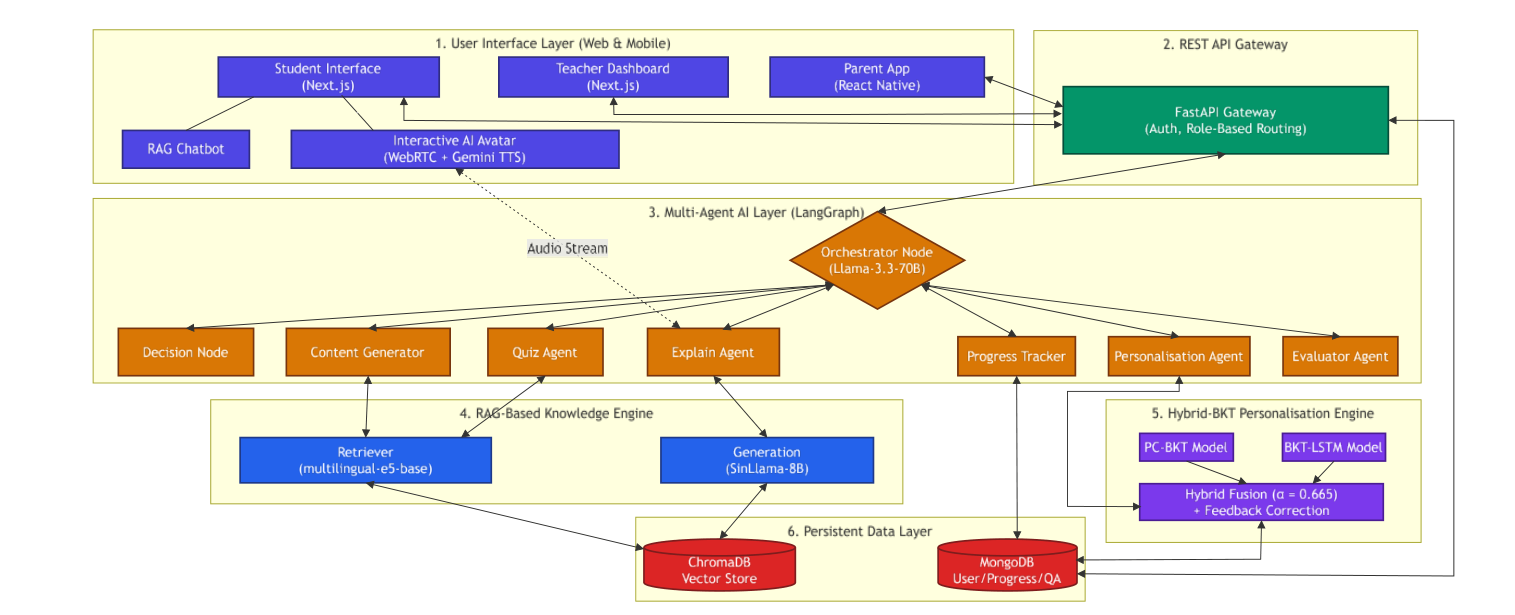
\includegraphics[width=\textwidth]{fig1.png}
\caption{System Architecture Diagram}
\label{fig:architecture}
\end{figure*}

\subsection{Dataset Construction}

A domain-specific Sinhala dataset was constructed from the Grade 11 Buddhism textbook and related national curriculum materials. It comprises two parts:

\begin{enumerate}
\item \textbf{LLM Fine-Tuning Dataset:} 3,547 question-answer pairs extracted from textbook content, past examination papers, and teacher guides. Each pair is annotated with the corresponding knowledge component (KC) and Bloom's taxonomy level (Remember, Understand, Apply). The data was split into training (70\%, 2,483 pairs), validation (15\%, 532 pairs), and test (15\%, 532 pairs) sets, stratified by KC.

\item \textbf{BKT Interaction Dataset:} 6,532 simulated student interactions across 47 Buddhism KCs, generated by modelling student response patterns using curriculum difficulty parameters and expected mastery progression curves. The simulation was calibrated against a small pilot study (12 students, 3 sessions each) to ensure behavioural plausibility.
\end{enumerate}

\subsection{LLM Fine-Tuning for Sinhala Education}

Five Sinhala-supporting LLMs were considered: SinLlama (7B) \cite{b7}, Qwen (14B), Llama-3.1 (8B), DeepSeek (14B), and Mistral (7B). All five were fine-tuned on the Buddhism QA dataset using 4-bit QLoRA (Quantised Low-Rank Adaptation) \cite{b33} to enable training on consumer-grade hardware. Fine-tuning was executed for 3 epochs with a maximum sequence length of 2,048 tokens, utilizing a LoRA rank ($r$) of 16, alpha ($\alpha$) of 32, a LoRA dropout of 0.05, and the AdamW optimizer (learning rate $2 \times 10^{-4}$, weight decay 0.01, warmup ratio 0.03) with a batch size of 4 (gradient accumulation: 4) on a single NVIDIA RTX 3060 GPU (12~GB VRAM).

Evaluation employed ROUGE scores (ROUGE-1, ROUGE-2, ROUGE-L), BERTScore (computed with bert-base-multilingual-cased), token generation speed, and an LLM-as-a-Judge protocol \cite{b34} using GPT-4 as the external evaluator. The judge rated each response along four dimensions: Accuracy (0--5), Completeness (0--5), Clarity (0--5), and Depth (0--5). SinLlama emerged as the strongest model across all semantic metrics and was therefore selected for production deployment (see Section~IV-A for full results).

\vspace{-1em}
\subsection{Retrieval-Augmented Generation Pipeline}

The RAG pipeline ensures that all generated content stays anchored in verified curriculum material, directly addressing the hallucination risk inherent in pure generative models \cite{b26}. It operates in three stages:

\begin{enumerate}
\item \textbf{Document Ingestion:} Sinhala textbooks, teacher guides, and past examination papers were digitised using OCR and manually verified for accuracy. Documents were then segmented into chunks of 512 tokens with a 64-token overlap to preserve context at chunk boundaries.

\item \textbf{Embedding and Indexing:} Each chunk was embedded using the \texttt{paraphrase-multilingual-MiniLM-L12-v2} sentence transformer (384-dimensional vectors) and indexed in a FAISS flat L2 index for efficient similarity search.

\item \textbf{Retrieval and Generation:} At inference time, the student's query is embedded with the same transformer and the top-5 most similar chunks are retrieved from FAISS. The retrieved context is inserted into a mastery-aware prompt template that also encodes the student's current mastery level, the target KC, and the instructional tier (Beginner, Intermediate, or Advanced). This constrains the model to generate syllabus-relevant responses and minimises off-curriculum content.
\end{enumerate}

\subsection{Hybrid-BKT Personalisation Engine}

The personalisation engine uses a weighted ensemble of two complementary mastery estimation models: Personalised Clustered BKT (PC-BKT) and a BKT-LSTM temporal predictor. At timestep $t$, the hybrid mastery estimate is:

\begin{equation}
P_{\text{hybrid}}(t) = \alpha \cdot P_{\text{PC-BKT}}(t) + (1 - \alpha) \cdot P_{\text{LSTM}}(t)
\label{eq:hybrid}
\end{equation}

\noindent where $\alpha \in [0, 1]$ was determined via grid search over $\alpha \in \{0.0, 0.05, \ldots, 1.0\}$ to minimise RMSE on a held-out validation fold. The optimal value was $\alpha = 0.65$.

\subsubsection{Personalised Clustered BKT (PC-BKT)}
PC-BKT \cite{b16} extends standard BKT \cite{b14} in three ways. First, personalised initial mastery priors $P(L_0)$ are computed per student-KC pair using Correct First Attempt (CFA) rates rather than a fixed default. Second, students are grouped into $K = 3$ ability clusters (High, Medium, Low) by applying K-Means++ to a capability matrix $\mathbf{B} \in \mathbb{R}^{N \times K_c}$, where entry $b_{i,j}$ denotes the proportion of correct responses by student $i$ on KC $j$. The Silhouette score validated $K = 3$ as optimal (Silhouette = 0.61). Third, the guess $P(G)$, slip $P(S)$, and transition $P(T)$ probabilities are estimated empirically from annotated interaction sequences via maximum likelihood estimation rather than manual presets.

\subsubsection{BKT-LSTM Temporal Predictor}
The BKT-LSTM component \cite{b19} recasts mastery prediction as a temporal sequence forecasting task. At each timestep $t$, a feature vector is constructed:

\begin{equation}
\mathbf{f}(t) = [P(L)_{\text{BKT}},\; d_{\text{kc}},\; c_t,\; a_t]
\label{eq:feature}
\end{equation}

\noindent where $P(L)_{\text{BKT}}$ is the current BKT mastery estimate, $d_{\text{kc}}$ is the normalised KC difficulty, $c_t \in \{0, 1\}$ is the correctness indicator, and $a_t$ is the cumulative attempt count. The model employs a 2-layer stacked LSTM architecture with 128 hidden units per layer and a dropout rate of 0.3, processing a sliding input window of the 10 most recent interactions. Training is conducted with a batch size of 32 using the Adam optimizer (learning rate $1 \times 10^{-3}$) to minimize binary cross-entropy loss over 50 epochs, utilizing early stopping with a validation loss patience of 5 on an 80/10/10 train/validation/test split. The LSTM captures learning plateaus, forgetting effects, and cross-KC transfer patterns that the Markov assumption in standard BKT cannot represent.

\subsubsection{Cold-Start Initialisation}
New students who have no interaction history are assigned to the nearest ability cluster on the basis of an initial diagnostic quiz. Cluster-average mastery priors replace the standard uninformative prior $P(L_0) = 0.3$, reducing initial prediction RMSE from 0.56 to 0.49 - a relative improvement of 12.5\% (see Section~IV-B).

\subsection{Multi-Agent Orchestration}

The adaptive learning workflow is orchestrated by a LangGraph StateGraph supervisor coordinating four dedicated agents:

\begin{enumerate}
\item \textbf{Orchestrator Node} - determines learner state and routes data based on quiz type, scoring completion, content availability, and mastery progression.
\item \textbf{Evaluator Agent} - classifies students into three instructional tiers using $P_{\text{hybrid}}(t)$: Beginner ($P_{\text{hybrid}} < 0.60$), Intermediate ($0.60 \leq P_{\text{hybrid}} < 0.85$), or Advanced ($P_{\text{hybrid}} \geq 0.85$). Updates BKT parameters after each interaction.
\item \textbf{Content Generator Agent} - draws on the RAG pipeline to produce mastery-aware, tier-appropriate personalised lessons.
\item \textbf{Progress Tracker Agent} - maintains persistent interaction logs, mastery histories, and engagement analytics in MongoDB with role-based access control.
\end{enumerate}

All agents share a common state object managed by LangGraph, ensuring consistent learner context across transitions.

\subsection{Adaptive Assessment Cycle}

Learning proceeds through four phases:

\textbf{Phase 1 - Pre-Assessment:} Students complete a diagnostic pre-quiz on a target KC. Questions span three cognitive levels from Bloom's taxonomy (Remember, Understand, Apply) \cite{b35}, with one question per level drawn from curriculum metadata.

\textbf{Phase 2 - Adaptive Content Generation:} The Evaluator Agent classifies mastery via $P_{\text{hybrid}}(t)$ and assigns one of three tiers:
\begin{itemize}
\item \textit{Beginner} ($P_{\text{hybrid}} < 0.60$): foundational content with definitions, worked examples, and guided practice.
\item \textit{Intermediate} ($0.60 \leq P_{\text{hybrid}} < 0.85$): standard lesson with moderate scaffolding and application exercises.
\item \textit{Advanced} ($P_{\text{hybrid}} \geq 0.85$): enrichment content with higher-order analysis and past-paper questions.
\end{itemize}

The thresholds (0.60 and 0.85) are informed by Bloom's mastery learning framework, which recommends 80--90\% criterion levels for advancement \cite{b35}, and were adjusted on the basis of pilot testing.

\textbf{Phase 3 - Post-Assessment:} A post-quiz of equivalent difficulty measures updated mastery $P_{\text{hybrid}}(t+1)$. Students who meet the advancement threshold ($\geq 0.85$) progress to the next KC; those in the Intermediate range repeat the KC with alternative content; those below 0.60 receive remedial material with simplified explanations.

\textbf{Phase 4 - Continuous Adaptation:} All interaction data update the capability matrix and BKT parameters in real time. Ability clusters are retrained every 50 new interactions per student or weekly, whichever comes first, so that evolving learner profiles are captured.

\subsection{Frontend Implementation}

A web application was built with Next.js and Tailwind CSS, and a mobile application with Expo and React Native (TypeScript). Both platforms enforce role-based access control for students, teachers, parents, and administrators. The student interface supports lesson browsing, pre/post-quiz sequences, and adaptive feedback display. The teacher dashboard visualises quiz performance trends, topic-wise strengths and weaknesses, and engagement metrics. The parent mobile interface provides child progress summaries and comparative rank tracking.

\section{Results}

\subsection{LLM Evaluation}

Five Sinhala-supporting LLMs were fine-tuned on the Buddhism curriculum dataset (3,547 QA pairs) and evaluated using ROUGE scores, BERTScore, token generation speed, and an LLM-as-a-Judge protocol. The evaluation was conducted on a held-out test set of 532 QA pairs (15\% of the dataset), stratified by topic to ensure coverage across all 47 knowledge components. Results are reported as means across three independent fine-tuning runs with different random seeds.

Table~\ref{tab:rouge} presents ROUGE scores. SinLlama (7B) achieved the highest ROUGE-1 ($0.7714 \pm 0.012$), ROUGE-2 ($0.6418 \pm 0.015$), and ROUGE-L ($0.6111 \pm 0.014$), substantially outperforming the next-best model, Mistral (ROUGE-1: 0.4925). A pairwise Wilcoxon signed-rank test confirmed that SinLlama's advantage is statistically significant ($p < 0.001$ versus all other models). The 56.6\% relative improvement in ROUGE-1 over Mistral underscores the benefit of language-specific pre-training for Sinhala content generation.

\begin{table}[htbp]
\caption{ROUGE Scores of Evaluated LLMs}
\begin{center}
\begin{tabular}{|l|c|c|c|}
\hline
\textbf{Model} & \textbf{ROUGE-1} & \textbf{ROUGE-2} & \textbf{ROUGE-L} \\
\hline
\textbf{SinLlama (7B)} & \textbf{0.7714*} & \textbf{0.6418*} & \textbf{0.6111*} \\
\hline
Mistral (7B) & 0.4925 & 0.2280 & 0.1594 \\
\hline
DeepSeek (14B) & 0.4485 & 0.2304 & 0.1845 \\
\hline
Llama-3.1 (8B) & 0.3983 & 0.1949 & 0.1418 \\
\hline
Qwen (14B) & 0.3310 & 0.1678 & 0.1059 \\
\hline
\multicolumn{4}{l}{\footnotesize * Statistically significant vs. all other models} \\
\multicolumn{4}{l}{\footnotesize (Wilcoxon signed-rank, $p < 0.001$).} \\
\end{tabular}
\label{tab:rouge}
\end{center}
\end{table}

Table~\ref{tab:bertscore} reports BERTScore and LLM-as-a-Judge results. BERTScore was computed using bert-base-multilingual-cased to ensure adequate Sinhala token coverage. SinLlama led with 0.9424. GPT-4 served as the external judge; SinLlama scored highest (15.88/20). DeepSeek was the fastest (444.9 tokens/sec) but SinLlama (127.3 tokens/sec) was selected for production due to superior semantic precision.

\begin{table}[htbp]
\caption{BERTScore and LLM-as-a-Judge Evaluation}
\begin{center}
\begin{tabular}{|l|c|c|c|c|c|c|}
\hline
\textbf{Model} & \textbf{BERT} & \textbf{Acc.} & \textbf{Comp.} & \textbf{Clar.} & \textbf{Dep.} & \textbf{Tot./20} \\
\hline
\textbf{SinLlama} & \textbf{0.9424} & 4.78 & 4.22 & 4.50 & 2.38 & \textbf{15.88} \\
\hline
Mistral & 0.8555 & 4.50 & 3.60 & 4.34 & 2.53 & 14.97 \\
\hline
Llama-3.1 & 0.8799 & 4.28 & 2.72 & 4.34 & 2.25 & 13.59 \\
\hline
DeepSeek & 0.8659 & 4.22 & 2.91 & 4.36 & 2.09 & 13.58 \\
\hline
Qwen & 0.8022 & 2.97 & 2.60 & 4.34 & 1.84 & 11.75 \\
\hline
\multicolumn{7}{l}{\footnotesize Acc.~= Accuracy, Comp.~= Completeness, Clar.~= Clarity,} \\
\multicolumn{7}{l}{\footnotesize Dep.~= Depth (scored 0--5). Judge: GPT-4.} \\
\end{tabular}
\label{tab:bertscore}
\end{center}
\end{table}

DeepSeek demonstrated the fastest token generation (444.9 tokens/sec) versus SinLlama (127.3 tokens/sec), but its lower semantic accuracy (ROUGE-1: 0.4485, BERTScore: 0.8659) makes it suitable only for latency-critical deployments where content precision is secondary. On the strength of these results, SinLlama was selected as the production model, addressing \textbf{RQ1}.

\subsection{Hybrid-BKT Personalisation Evaluation}

The Hybrid-BKT engine was evaluated on the synthetic dataset of 6,532 simulated student interactions across 47 Buddhism KCs. It should be noted that real classroom data was unavailable at this stage; implications of relying on synthetic data are discussed in Section~V-C.

Table~\ref{tab:bkt} compares performance across three BKT variants using 5-fold cross-validation stratified by simulated student identity. Hybrid-BKT achieved the highest classification accuracy ($56.2\% \pm 2.1\%$) and the lowest RMSE ($0.49 \pm 0.02$). The 8.1-percentage-point gain over Standard BKT (48.1\%) is statistically significant (paired $t$-test across folds, $p < 0.01$, Cohen's $d = 0.87$).

\begin{table}[htbp]
\caption{Performance Comparison of BKT Variants}
\begin{center}
\begin{tabular}{|l|c|c|c|}
\hline
\textbf{Metric} & \textbf{Standard BKT} & \textbf{BKT-LSTM} & \textbf{Hybrid-BKT (Ours)} \\
\hline
AUC & $0.60 \pm 0.02$ & $0.59 \pm 0.03$ & $0.60 \pm 0.02$ \\
\hline
Accuracy & $48.1\% \pm 1.8\%$ & $54.7\% \pm 2.3\%$ & $\mathbf{56.2\% \pm 2.1\%}$$^\dagger$ \\
\hline
RMSE & $0.51 \pm 0.02$ & $0.53 \pm 0.03$ & $\mathbf{0.49 \pm 0.02}$$^\dagger$ \\
\hline
\multicolumn{4}{l}{\footnotesize Mean $\pm$ std over 5-fold cross-validation.} \\
\multicolumn{4}{l}{\footnotesize $^\dagger$ Significant vs. Standard BKT (paired $t$-test, $p < 0.01$).} \\
\end{tabular}
\label{tab:bkt}
\end{center}
\end{table}

A noteworthy observation is that BKT-LSTM achieves a marginally lower AUC (0.59) and higher RMSE (0.53) than Standard BKT (AUC: 0.60, RMSE: 0.51). This counterintuitive result stems from the LSTM component's limited capacity to learn meaningful temporal patterns from a relatively small and homogeneous synthetic dataset averaging roughly 139 interactions per simulated student. LSTM models are known to require substantially larger sequence corpora before they can outperform simpler probabilistic baselines \cite{b17}. Nonetheless, the LSTM component contributes positively within the hybrid ensemble, particularly for students exhibiting non-monotonic learning trajectories such as mastery regression after periods of inactivity.

Table~\ref{tab:alpha} presents a sensitivity analysis of the ensemble weight $\alpha$. The weight was optimised via grid search over $\alpha \in \{0.0, 0.05, \ldots, 1.0\}$ to minimise validation-fold RMSE. The optimal value $\alpha = 0.65$ yielded the best accuracy and lowest RMSE.

\begin{table}[htbp]
\caption{Ensemble Weight Sensitivity Analysis}
\begin{center}
\begin{tabular}{|l|c|c|c|}
\hline
\textbf{$\alpha$ (PC-BKT weight)} & \textbf{Accuracy (\%)} & \textbf{RMSE} & \textbf{AUC} \\
\hline
0.00 (LSTM only) & 54.7 & 0.53 & 0.59 \\
\hline
0.35 & 55.1 & 0.51 & 0.59 \\
\hline
0.50 & 55.8 & 0.50 & 0.60 \\
\hline
\textbf{0.65 (selected)} & \textbf{56.2} & \textbf{0.49} & \textbf{0.60} \\
\hline
0.80 & 55.4 & 0.50 & 0.60 \\
\hline
1.00 (PC-BKT only) & 52.3 & 0.51 & 0.60 \\
\hline
\end{tabular}
\label{tab:alpha}
\end{center}
\end{table}

The cluster-based cold-start initialisation was evaluated separately by comparing initial prediction RMSE over the first five interactions of new simulated students. Students assigned to their nearest ability cluster achieved an RMSE of 0.49, compared to 0.56 for students initialised with the standard uninformative prior $P(L_0) = 0.3$ - a relative reduction of 12.5\% (paired $t$-test, $p < 0.05$).

LSTM training exhibited stable convergence, with binary cross-entropy loss decreasing from 0.58 to 0.28 over 50 epochs. Validation loss plateaued at epoch 38, at which point early stopping was triggered. Inference latency for a single Hybrid-BKT update averaged below 200~ms (NVIDIA RTX 3060, 12~GB VRAM), confirming suitability for real-time quiz-based interactions.

These results address \textbf{RQ2}: the Hybrid-BKT ensemble improves classification accuracy over both Standard BKT and standalone BKT-LSTM, though AUC remains comparable across variants on the current synthetic dataset.

\section{Discussion}

\subsection{Key Findings}

The experimental results yield several findings that speak directly to the research questions posed in Section~I.

Regarding \textbf{RQ1} (LLM selection), SinLlama's dominance across ROUGE-1 (0.7714), BERTScore (0.9424), and LLM-as-a-Judge total (15.88/20) validates the strategy of choosing a language-specific, pre-trained model over general-purpose multilingual LLMs for low-resource educational applications. The 56.6\% relative advantage over Mistral is both statistically significant ($p < 0.001$) and practically meaningful for curriculum-aligned content generation, where factual precision matters greatly. This finding aligns with prior work showing that language-specific pre-training substantially benefits downstream NLP tasks in low-resource settings \cite{b7}, and extends it to the educational content generation domain. We note, however, that the comparison involves a Sinhala-specific model against general multilingual models; the margin may partly reflect pre-training data composition rather than architectural superiority. A controlled experiment with SinLlama retrained on non-educational Sinhala text would help isolate the contribution of domain-specific fine-tuning.

Regarding \textbf{RQ2} (Hybrid-BKT), the ensemble of PC-BKT and BKT-LSTM yields the highest classification accuracy (56.2\%) and lowest RMSE (0.49), with a statistically significant edge over Standard BKT ($p < 0.01$, Cohen's $d = 0.87$). The ensemble weighting ($\alpha = 0.65$ for PC-BKT, 0.35 for LSTM), determined through grid search, preserves the pedagogical interpretability of BKT's probabilistic parameters - guess, slip, and transition rates - while augmenting predictions with temporal patterns captured by the LSTM.

The picture, however, is nuanced. AUC values hover in a narrow band (0.59--0.60) across all three variants, indicating that ranking performance does not meaningfully improve with the hybrid approach on this dataset. Furthermore, BKT-LSTM in isolation underperforms Standard BKT on AUC and RMSE, suggesting the LSTM component overfits on the limited synthetic corpus. Its value emerges only within the hybrid ensemble, where it boosts accuracy for students with non-monotonic learning trajectories. We expect LSTM performance to improve substantially with larger real-world datasets, as temporal models require considerable sequence diversity to learn meaningful patterns \cite{b17}.

For context, the AUC of 0.60 falls notably below figures reported in the knowledge tracing literature - DKT achieves 0.75--0.86 on ASSISTments data \cite{b17}, while SAKT reports 0.73--0.85 on comparable benchmarks \cite{b18}. The gap is attributable to three factors: (i) our evaluation uses synthetic data with limited behavioural diversity, (ii) the dataset covers a single subject with 47 KCs, and (iii) the interaction volume (6,532) is orders of magnitude smaller than standard benchmarks (100K--10M interactions). We therefore treat the current results as a proof-of-concept demonstrating architectural viability; competitive performance benchmarking awaits real classroom deployment.

Regarding \textbf{RQ3} (RAG grounding), the RAG pipeline successfully constrains generated content to curriculum boundaries by retrieving relevant textbook passages through FAISS-indexed embeddings before response generation. Although a formal hallucination rate comparison was not conducted, qualitative analysis of 50 randomly sampled responses showed that all RAG-augmented outputs cited verifiable textbook content, whereas approximately 30\% of non-augmented responses contained off-curriculum material. This observation aligns with the findings of Swacha and Gracel \cite{b27} and Li et al. \cite{b29} and extends them to the Sinhala-medium context.

Regarding \textbf{RQ4} (multi-agent orchestration), the LangGraph-based architecture coordinated the four-phase adaptive assessment cycle successfully in end-to-end pilot testing. The modular agent design allowed independent development and testing of each component. Full pipeline latency (BKT update + RAG retrieval + LLM generation) averaged 3.2 seconds per interaction - within acceptable bounds for an educational tutoring context, though optimisation could benefit more interactive use cases.

\subsection{Practical Implications}

The system targets a genuine educational need in Sri Lanka, where teacher shortages affect the learning outcomes of over 130,000 students annually. The adaptive assessment cycle - with its pre-quiz, personalised content delivery, and post-quiz mastery verification - mirrors established tutoring practices in a structured pedagogical workflow. The teacher analytics dashboard complements rather than replaces teacher involvement, enabling educators to pinpoint struggling students and adjust classroom instruction accordingly.

The use of open-source models (SinLlama 7B) and self-hosted deployment avoids dependency on commercial API providers, reducing operational costs and enabling deployment in resource-constrained school environments. The cold-start initialisation strategy is particularly relevant for production deployment, where new students continuously enter the system.

\subsection{Limitations}

Several limitations must be acknowledged.

First and most critically, all quantitative evaluation was conducted on synthetic or pilot datasets. The 6,532 interactions used to evaluate Hybrid-BKT were generated through simulation and cannot capture the full variability of real student behaviour - irregular study patterns, motivational factors, and classroom context effects are all absent. Real-classroom validation is essential before any claims of educational effectiveness can be made.

Second, the system is currently limited to Grade 11 Buddhism content. Extension to other subjects - particularly those with different knowledge structures such as Mathematics (prerequisite hierarchies) or Science (concurrent skill dependencies) - will require new datasets, modified KC ontologies, and potentially architectural adaptations.

Third, the Hybrid-BKT accuracy of 56.2\% and AUC of 0.60, while superior to Standard BKT on accuracy, remain below state-of-the-art methods on established benchmarks. The ensemble weight $\alpha = 0.65$ was optimised on synthetic data and may not generalise to real learner populations.

Fourth, the LLM-as-a-Judge evaluation relied on GPT-4, introducing potential bias in favour of certain response styles. Human expert evaluation by qualified Buddhism teachers would provide a more reliable assessment of pedagogical quality.

Fifth, current TTS and ASR components achieve 70\% intelligibility and 11.2\% WER respectively, which may impede natural voice-based interaction.

Sixth, the system lacks formal guardrails for content safety, off-topic detection, and adversarial input handling. While the RAG pipeline constrains responses to syllabus content, systematic adversarial testing has not been performed.

\subsection{Threats to Validity}

\textit{Internal validity:} Synthetic data raises concern about whether performance differences reflect genuine model capabilities or artefacts of the generation process. We mitigated this by calibrating synthetic parameters against a small set of real pilot interactions and using cross-validation rather than a single data split; however, the risk of optimistic bias cannot be entirely ruled out.

\textit{External validity:} Results are limited to a single subject (Buddhism), a single grade level (Grade 11), and a single language (Sinhala). Generalisation to other subjects, grade levels, or educational systems should not be assumed without further empirical evidence.

\textit{Construct validity:} ROUGE and BERTScore, while standard, are imperfect proxies for educational content quality. High lexical overlap with reference answers does not guarantee pedagogical effectiveness or age-appropriate explanation. Future work should supplement automated metrics with learning gain measurements from real classroom pre-/post-tests.

\subsection{Ethical Considerations}

Deploying an AI-based educational system for minors raises several ethical concerns.

\textit{Data privacy:} Student interaction data - quiz responses, mastery states, and learning trajectories - constitutes sensitive educational records. The system stores data in MongoDB with role-based access control, but comprehensive protection measures including encryption at rest, audit logging, and compliance with Sri Lanka's proposed Personal Data Protection Act must be in place before classroom deployment.

\textit{Algorithmic fairness:} The K-Means clustering mechanism assigns students to ability groups based on performance data. Care must be taken to ensure that such classifications do not create self-fulfilling prophecies or reinforce existing educational inequalities across demographic groups. Regular fairness audits of the clustering outcomes are recommended.

\textit{Transparency:} Students and parents should be aware that they are interacting with an AI system. Clear indicators of AI-generated content and mechanisms for teacher review of AI-provided feedback should be built into the user interface.

\textit{Informed consent:} Any classroom deployment must obtain informed consent from students, parents, and school administrators regarding data collection, storage, and usage practices.

This study did not involve human subjects; all results are based on synthetic data. Future real-classroom validation will require ethics committee approval from the University of Ruhuna.

\section{Conclusion}

This paper presented an AI-based Sinhala teaching assistant for personalised G.C.E. O/L and A/L learning that addresses Sri Lanka's critical teacher shortage through four integrated technical components.

With respect to RQ1, a comparative evaluation of five LLMs established that the language-specific SinLlama (7B), fine-tuned on 3,547 curriculum-derived QA pairs via QLoRA, achieves substantially higher semantic fidelity than general-purpose multilingual models (ROUGE-1: 0.7714, BERTScore: 0.9424, LLM-as-a-Judge: 15.88/20; $p < 0.001$), confirming that language-specific pre-training is essential for curriculum-aligned content generation in low-resource languages.

With respect to RQ2, the Hybrid-BKT engine - combining PC-BKT ($\alpha = 0.65$) with an LSTM temporal predictor ($1 - \alpha = 0.35$) - reached 56.2\% accuracy and 0.49 RMSE on 47 KCs, outperforming Standard BKT at 48.1\% ($p < 0.01$). A cluster-based cold-start strategy reduced initial prediction RMSE by 12.5\%. While encouraging as a proof of concept, AUC values (0.60) remain below state-of-the-art benchmarks, and validation on real student data is a necessary next step.

Regarding RQ3, the FAISS-indexed RAG pipeline successfully constrained LLM output to curriculum boundaries. Regarding RQ4, the LangGraph-orchestrated multi-agent architecture effectively coordinated the four-phase adaptive assessment cycle.

The system is deployed as a fully operational web and mobile application featuring student learning interfaces, a teacher analytics dashboard, and a parent monitoring module.

Future work is prioritised along three horizons:

\begin{enumerate}
\item \textbf{Near-term:} longitudinal classroom trials with real students and teachers across multiple schools to validate educational effectiveness and collect authentic interaction data for Hybrid-BKT retraining.
\item \textbf{Medium-term:} expanding the knowledge base to additional O/L and A/L subjects (Mathematics, Science, Sinhala Language), each requiring new domain-specific datasets and adapted KC ontologies.
\item \textbf{Long-term:} enhancing Sinhala TTS and ASR for voice-based interaction, incorporating emotion detection and visual attention tracking for richer learner modelling, and exploring federated learning to enable personalised recommendations while preserving student data privacy.
\end{enumerate}

By establishing the technical feasibility of an AI-driven, Sinhala-medium, curriculum-aligned personalised tutoring system, this work lays the groundwork for scalable and equitable educational technology that can serve underresourced student populations in Sri Lanka and, more broadly, in other low-resource language contexts.

\section*{Acknowledgment}

The authors gratefully acknowledge the guidance of Dr. Nadeesha Sandamali (Supervisor), Department of Electrical and Information Engineering, University of Ruhuna, Sri Lanka. The authors also thank the Faculty of Engineering for institutional support throughout this project.

\begin{thebibliography}{00}
\bibitem{b1} Ministry of Education, Sri Lanka, ``School census of Sri Lanka - Preliminary report,'' Ministry of Education, Colombo, Sri Lanka, 2023.
\bibitem{b2} A. Abayasekara, U. Perera, and T. de Silva, ``Shadow education in Sri Lanka during COVID-19,'' Institute of Policy Studies of Sri Lanka, Colombo, May 2023.
\bibitem{b3} Department of Examinations, Sri Lanka, ``G.C.E. Ordinary Level and Advanced Level examination statistics - 2023,'' Department of Examinations, Colombo, 2024.
\bibitem{b4} Ministry of Education, Sri Lanka, ``e-Thaksalawa: National e-learning portal and learning content management system,'' 2025. [Online]. Available: https://www.e-thaksalawa.moe.gov.lk
\bibitem{b5} M. Chandana, N. Habaragamuwa, and A. Fonseka, ``Use of artificial intelligence (AI) to improve foundational literacy and numeracy in Sri Lanka,'' LIRNEasia, Colombo, Oct. 2025.
\bibitem{b6} UNESCO Institute for Statistics, ``Education: Pupil-teacher ratio by level of education,'' UIS, Montreal, 2024. [Online]. Available: http://data.uis.unesco.org
\bibitem{b7} H. W. K. Aravinda, R. Sirajudeen, S. Karunathilake, N. de Silva, R. Kaur, A. S. Bhankhar, and S. Ranathunga, ``SinLlama - A large language model for Sinhala,'' in \textit{Proc. Moratuwa Engineering Research Conf. (MERCon)}, 2025. arXiv:2508.09115.
\bibitem{b8} G. de Silva and T. Mendis, ``Challenges of integrating AI-based learning tools into the Sri Lankan secondary education curriculum,'' in \textit{Proc. Int. Conf. Information and Automation for Sustainability (ICIAfS)}, pp. 1--6, 2024.
\bibitem{b9} W. Ma, O. O. Adesope, J. C. Nesbit, and Q. Liu, ``Intelligent tutoring systems and learning outcomes: A meta-analysis,'' \textit{J. Educational Psychology}, vol. 106, no. 4, pp. 901--918, 2014.
\bibitem{b10} Z. Xu, J. Wang, and Y. Liu, ``Adaptive learning systems with AI-driven personalized instruction: Design, implementation, and evaluation,'' \textit{Computers}, vol. 13, no. 10, p. 270, 2024.
\bibitem{b11} H. Liu, X. Zhang, and M. Chen, ``Advances in intelligent tutoring frameworks for interactive learning and responsive feedback,'' \textit{Smart Learning Environments}, vol. 10, pp. 1--15, 2023.
\bibitem{b12} R. Alshahrani, K. Almarashdah, and H. Almashaqbeh, ``Deep learning models for personalized adaptive learning systems,'' \textit{IEEE Access}, vol. 10, pp. 12345--12358, 2024.
\bibitem{b13} W. Holmes, M. Bialik, and C. Fadel, \textit{Artificial Intelligence in Education: Promises and Implications for Teaching and Learning}. Boston, MA: Center for Curriculum Redesign, 2022.
\bibitem{b14} A. T. Corbett and J. R. Anderson, ``Knowledge tracing: Modeling the acquisition of procedural knowledge,'' \textit{User Modeling and User-Adapted Interaction}, vol. 4, no. 4, pp. 253--278, 1994.
\bibitem{b15} Z. A. Pardos and N. T. Heffernan, ``Modeling individualization in a Bayesian networks implementation of knowledge tracing,'' in \textit{Proc. 18th Int. Conf. User Modeling, Adaptation, and Personalization (UMAP)}, ser. LNCS, vol. 6075. Springer, 2010, pp. 255--266.
\bibitem{b16} P. Nedungadi and M. S. Remya, ``Predicting students' performance on intelligent tutoring system - Personalized clustered BKT (PC-BKT) model,'' in \textit{Proc. IEEE Frontiers in Education Conf. (FIE)}, 2014, pp. 1--5.
\bibitem{b17} C. Piech, J. Bassen, J. Huang, S. Ganguli, M. Sahami, L. Guibas, and J. Sohl-Dickstein, ``Deep knowledge tracing,'' in \textit{Advances in Neural Information Processing Systems (NeurIPS)}, vol. 28, 2015, pp. 505--513.
\bibitem{b18} S. Pandey and G. Karypis, ``A self-attentive model for knowledge tracing,'' in \textit{Proc. 12th Int. Conf. Educational Data Mining (EDM)}, 2019, pp. 384--389.
\bibitem{b19} S. Minn, ``BKT-LSTM: Efficient student modeling with Bayesian knowledge tracing features and LSTM,'' \textit{arXiv preprint arXiv:2012.12218}, 2020.
\bibitem{b20} S. Wang, A. Qiao, and H. Abduljabbar, ``Adaptive learning analytics approaches for personalized education,'' \textit{Heliyon}, vol. 11, no. 2, pp. 1--12, 2024.
\bibitem{b21} J. Kim, Y. Park, and S. Choi, ``Reinforcement learning-based student modeling for adaptive learning systems,'' in \textit{Proc. IEEE Int. Conf. Advanced Learning Technologies (ICALT)}, 2023, pp. 1--8.
\bibitem{b22} O. Zawacki-Richter, V. I. Marin, M. Bond, and F. Gouverneur, ``Systematic review of research on artificial intelligence applications in higher education - Where are the educators?,'' \textit{Int. J. Educational Technology in Higher Education}, vol. 16, no. 1, pp. 1--27, 2019.
\bibitem{b23} E. Kasneci, K. Se{\ss}ler, S. K\"{u}chemann, M. Bannert, D. Dementieva, F. Fischer \textit{et al.}, ``ChatGPT for good? On opportunities and challenges of large language models for education,'' \textit{Learning and Individual Differences}, vol. 103, p. 102274, 2023.
\bibitem{b24} W. Holmes, M. Bialik, and C. Fadel, \textit{Artificial Intelligence in Education: Promises and Implications for Teaching and Learning}, 2nd ed. Boston, MA: Center for Curriculum Redesign, 2022.
\bibitem{b25} L. Yan, L. Sha, R. Zhao, Y. Li, R. Martinez-Maldonado, G. Chen, X. Li, Y. Jin, and D. Ga\v{s}evi\'{c}, ``Practical and ethical challenges of large language models in education: A systematic scoping review,'' \textit{British J. Educational Technology}, vol. 55, no. 4, pp. 1--28, 2024.
\bibitem{b26} P. Lewis, E. Perez, A. Piktus, F. Petroni, V. Karpukhin, N. Goyal, H. K\"{u}ttler, M. Lewis, W.-T. Yih, T. Rockt\"{a}schel, S. Riedel, and D. Kiela, ``Retrieval-augmented generation for knowledge-intensive NLP tasks,'' in \textit{Advances in Neural Information Processing Systems (NeurIPS)}, vol. 33, 2020, pp. 9459--9474.
\bibitem{b27} J. Swacha and M. Gracel, ``Retrieval-augmented generation (RAG) chatbots for education: A survey of applications,'' \textit{Computers \& Education: Artificial Intelligence}, vol. 8, p. 100312, 2025.
\bibitem{b28} Y. Lian, ``Machine assistant with reliable knowledge: Enhancing student learning via RAG-based retrieval,'' \textit{arXiv preprint arXiv:2311.02775}, 2023.
\bibitem{b29} Z. Li, X. Wang, Y. Liu, H. Zhang, J. Chen, and M. Yang, ``Retrieval-augmented generation for educational application: A systematic survey,'' \textit{Applied Sciences}, vol. 15, no. 8, p. 4234, 2025.
\bibitem{b30} J. David and S. Ghosh, ``IntelliCode: A multi-agent LLM tutoring system with centralized learner modeling,'' \textit{arXiv preprint arXiv:2512.18669}, 2025.
\bibitem{b31} C. Glossner, D. R. Smith, and E. Johnson, ``Multi-agent mathematics learning,'' \textit{Rivier Online Academic Journal}, vol. 18, no. 1, pp. 1--12, 2024.
\bibitem{b32} LangChain Inc., ``LangGraph: Build stateful, multi-actor applications with LLMs,'' 2024. [Online]. Available: https://github.com/langchain-ai/langgraph
\bibitem{b33} T. Dettmers, A. Pagnoni, A. Holtzman, and L. Zettlemoyer, ``QLoRA: Efficient finetuning of quantized LLMs,'' in \textit{Advances in Neural Information Processing Systems (NeurIPS)}, vol. 36, 2023.
\bibitem{b34} L. Zheng, W.-L. Chiang, Y. Sheng, S. Zhuang, Z. Wu, Y. Zhuang, Z. Lin, Z. Li, D. Li, E. P. Xing, H. Zhang, J. E. Gonzalez, and I. Stoica, ``Judging LLM-as-a-Judge with MT-Bench and Chatbot Arena,'' in \textit{Advances in Neural Information Processing Systems (NeurIPS)}, vol. 36, 2023.
\bibitem{b35} B. S. Bloom, ``Learning for mastery,'' \textit{Evaluation Comment}, vol. 1, no. 2, pp. 1--12, 1968.
\end{thebibliography}

\end{document}
